% ============================================================
%  Employee Management System -- Project Documentation
%  Team Magnum | Adamas University | CSE Dept.
% ============================================================
\documentclass[12pt,a4paper]{report}

%--- Encoding & Fonts
\usepackage[utf8]{inputenc}
\usepackage[T1]{fontenc}
\usepackage{lmodern}
\usepackage{microtype}

%--- Page Layout
\usepackage[a4paper,top=2.5cm,bottom=2.5cm,left=2.5cm,right=2.5cm,headheight=15pt]{geometry}

%--- Color
\usepackage[dvipsnames,table]{xcolor}
\definecolor{primaryblue}{HTML}{1A3C6E}
\definecolor{accentblue}{HTML}{2E6DB4}
\definecolor{lightblue}{HTML}{D6E8F7}
\definecolor{softgray}{HTML}{F4F6F9}
\definecolor{midgray}{HTML}{9AA3AF}
\definecolor{darktext}{HTML}{1C1C2E}
\definecolor{successgreen}{HTML}{1B7A4E}
\definecolor{warnyellow}{HTML}{B8860B}
\definecolor{nodeblue}{HTML}{CBE0F5}
\definecolor{nodegreen}{HTML}{C8EDCD}
\definecolor{nodeyellow}{HTML}{FFF3CD}
\definecolor{nodepurple}{HTML}{E8D5F5}

%--- Headers and Footers
\usepackage{fancyhdr}
\pagestyle{fancy}
\fancyhf{}
\fancyhead[L]{\small\textit{Employee Management System}}
\fancyhead[R]{\small\textit{Team Magnum}}
\fancyfoot[C]{\small\thepage}
\renewcommand{\headrulewidth}{0.4pt}

%--- Chapter / Section Titles
\usepackage{titlesec}
\titleformat{\chapter}[display]
  {\normalfont\bfseries\LARGE}
  {\small\MakeUppercase{\chaptertitlename}\ \thechapter}
  {8pt}{\LARGE}[\vspace{4pt}\titlerule]
\titlespacing*{\chapter}{0pt}{-20pt}{24pt}

\titleformat{\section}
  {\normalfont\bfseries\large}
  {\thesection}{0.8em}{}
  [\vspace{2pt}\hrule\vspace{2pt}]
\titlespacing*{\section}{0pt}{16pt}{8pt}

\titleformat{\subsection}
  {\normalfont\bfseries\normalsize}
  {\thesubsection}{0.7em}{}
\titlespacing*{\subsection}{0pt}{12pt}{4pt}

\titleformat{\subsubsection}
  {\normalfont\bfseries\small}
  {\thesubsubsection}{0.6em}{}
\titlespacing*{\subsubsection}{0pt}{10pt}{3pt}

%--- Tables
\usepackage{booktabs}
\usepackage{tabularx}
\usepackage{array}
\renewcommand{\arraystretch}{1.35}

%--- Lists
\usepackage{enumitem}
\setlist[itemize]{leftmargin=1.5em,itemsep=2pt,topsep=4pt}
\setlist[enumerate]{leftmargin=1.8em,itemsep=2pt,topsep=4pt}

%--- Graphics & TikZ
\usepackage{graphicx}
\usepackage{tikz}
\usetikzlibrary{shapes.geometric,shapes.symbols,arrows.meta,positioning,fit,calc,backgrounds}

%--- Captions
\usepackage{caption}
\captionsetup{labelfont=bf,textfont=it,skip=6pt,justification=centering}

%--- Hyperlinks
\usepackage{hyperref}
\hypersetup{colorlinks=false,hidelinks}

%--- Misc
\usepackage{parskip}
\setlength{\parskip}{5pt}
\usepackage{setspace}
\setstretch{1.15}

% ============================================================
%  GLOBAL TIKZ STYLES  (borders/arrows = black; fills = color)
% ============================================================
\tikzset{
  % Context diagram
  sysnode/.style={ellipse,draw=black,fill=nodeblue,minimum width=3.2cm,minimum height=1.6cm,align=center,font=\bfseries\small,line width=1.2pt},
  extnode/.style={rectangle,rounded corners=4pt,draw=black,fill=nodeyellow,minimum width=2.8cm,minimum height=0.9cm,align=center,font=\small,line width=0.8pt},
  arrowstd/.style={-{Stealth[length=6pt]},thick,draw=black},
  % Architecture
  layerbox/.style={rectangle,draw=black,fill=softgray,minimum width=13cm,minimum height=1.4cm,align=center,font=\bfseries\small,line width=1pt,rounded corners=3pt},
  modbox/.style={rectangle,rounded corners=4pt,draw=black,fill=nodeblue,minimum width=3.4cm,minimum height=0.9cm,align=center,font=\small,line width=0.8pt},
  dbcyl/.style={cylinder,shape border rotate=90,draw=black,fill=nodegreen,minimum height=1.3cm,minimum width=3.2cm,align=center,font=\small\bfseries,line width=1pt,aspect=0.3},
  % DFD
  dfdproc/.style={circle,draw=black,fill=nodeblue,minimum size=3cm,align=center,font=\bfseries\small,line width=1.2pt},
  dfdent/.style={rectangle,rounded corners=3pt,draw=black,fill=nodeyellow,minimum width=3cm,minimum height=1.1cm,align=center,font=\small,line width=0.8pt},
  % Use case
  ucbox/.style={ellipse,draw=black,fill=nodepurple,minimum width=4.5cm,minimum height=1.1cm,align=center,font=\small,line width=0.8pt},
  % Activity
  actbox/.style={rectangle,rounded corners=10pt,draw=black,fill=nodepurple,minimum width=4.5cm,minimum height=0.75cm,align=center,font=\small,line width=0.8pt},
  notebox/.style={rectangle,draw=black!50,fill=softgray,minimum width=4cm,minimum height=0.65cm,align=center,font=\footnotesize},
  % Sequence
  actorbox/.style={rectangle,draw=black,fill=nodeblue,minimum width=2.8cm,minimum height=0.75cm,align=center,font=\small\bfseries,line width=0.8pt,rounded corners=2pt},
  lifeline/.style={dashed,draw=black!60,thick},
  msgfwd/.style={-{Stealth[length=5pt]},thick,draw=black},
  msgrtn/.style={-{Stealth[length=5pt]},thick,draw=black,dashed}
}

% ============================================================
%  TITLE PAGE
% ============================================================
\title{%
  \vspace{2cm}
  {\rule{\linewidth}{1.5pt}}\\[0.6cm]
  {\bfseries\Huge Employee Management System}\\[0.3cm]
  {\large\itshape Project Documentation \& Software Requirements Specification}\\[0.6cm]
  {\rule{\linewidth}{1.5pt}}\\[0.4cm]
  {\normalsize Adamas University \textbar\ Computer Science \& Engineering Department}
}
\author{%
  \vspace{0.5cm}
  {\large\bfseries Team Magnum}\\[0.4cm]
  \begin{tabular}{ll}
    \textbf{Souradeep Pradhan}           & Team Leader \\
    \textbf{Srijit Paul}                 & Frontend Developer \\
    \textbf{Aniruddha Das}               & Backend Developer \\
    \textbf{Asmita Mishra \& Anisha Dan} & Data Analysts \\
    \textbf{Soubhik Dutta}               & Database Manager \\
  \end{tabular}
}
\date{\today}

\begin{document}

\maketitle
\thispagestyle{empty}
\newpage
\tableofcontents
\newpage

% ============================================================
\chapter{Lab Showcase Details}
% ============================================================

\section{Project Title}
\textbf{Employee Management System (EMS)}

\section{Team Members}
\begin{itemize}
  \item \textbf{Souradeep Pradhan} \hfill \textit{Team Leader}
  \item \textbf{Srijit Paul} \hfill \textit{Frontend Developer}
  \item \textbf{Aniruddha Das} \hfill \textit{Backend Developer}
  \item \textbf{Asmita Mishra \& Anisha Dan} \hfill \textit{Data Analysts}
  \item \textbf{Soubhik Dutta} \hfill \textit{Database Manager}
\end{itemize}
Developed by \textbf{Team Magnum}, Computer Science \& Engineering Department, Adamas University.

\section{Aim}
To design and develop a unified platform that seamlessly bridges \textit{Core HR Operations} with \textit{Work Management} features --- automating workflows, reducing manual synchronisation overhead, and providing a centralised, authoritative repository for all employee data.

\section{Problem Statement}
Organisations relying on fragmented, paper-based HR systems suffer from data inconsistencies, slow retrieval, and error-prone manual processes. The EMS directly addresses this by replacing disconnected systems with a single, integrated platform that makes employee information easy to \textbf{store}, \textbf{update}, \textbf{search}, and \textbf{retrieve}, while enforcing data integrity at every step.

\section{System Context Diagram}

\begin{figure}[h!]
\centering
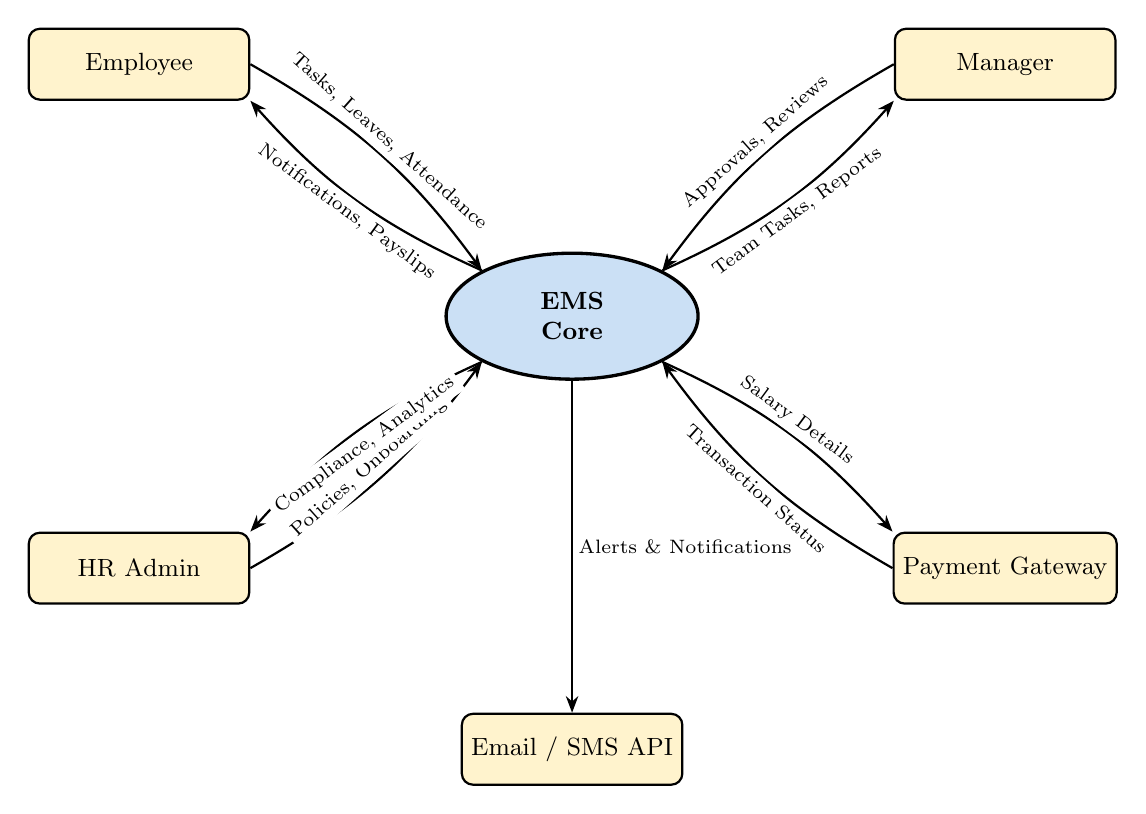
\begin{tikzpicture}
  \node[sysnode] (sys) at (0,0) {EMS\\Core};
  \node[extnode] (emp)     at (-5.5,  3.2) {Employee};
  \node[extnode] (mgr)     at ( 5.5,  3.2) {Manager};
  \node[extnode] (hradmin) at (-5.5, -3.2) {HR Admin};
  \node[extnode] (pay)     at ( 5.5, -3.2) {Payment Gateway};
  \node[extnode] (email)   at (  0,  -5.5) {Email / SMS API};
  % Employee <-> EMS
  \draw[arrowstd,bend left=12] (emp.east) to
    node[above,sloped,font=\scriptsize,fill=white,inner sep=2pt]{Tasks, Leaves, Attendance}
    (sys.north west);
  \draw[arrowstd,bend left=12] (sys.north west) to
    node[below,sloped,font=\scriptsize,fill=white,inner sep=2pt]{Notifications, Payslips}
    (emp.south east);
  % Manager <-> EMS
  \draw[arrowstd,bend right=12] (mgr.west) to
    node[above,sloped,font=\scriptsize,fill=white,inner sep=2pt]{Approvals, Reviews}
    (sys.north east);
  \draw[arrowstd,bend right=12] (sys.north east) to
    node[below,sloped,font=\scriptsize,fill=white,inner sep=2pt]{Team Tasks, Reports}
    (mgr.south west);
  % HR Admin <-> EMS
  \draw[arrowstd,bend right=12] (hradmin.east) to
    node[above,sloped,font=\scriptsize,fill=white,inner sep=2pt]{Policies, Onboarding}
    (sys.south west);
  \draw[arrowstd,bend right=12] (sys.south west) to
    node[below,sloped,font=\scriptsize,fill=white,inner sep=2pt]{Compliance, Analytics}
    (hradmin.north east);
  % Payment <-> EMS
  \draw[arrowstd,bend left=12] (sys.south east) to
    node[above,sloped,font=\scriptsize,fill=white,inner sep=2pt]{Salary Details}
    (pay.north west);
  \draw[arrowstd,bend left=12] (pay.west) to
    node[below,sloped,font=\scriptsize,fill=white,inner sep=2pt]{Transaction Status}
    (sys.south east);
  % Email (one-way)
  \draw[arrowstd] (sys.south) to
    node[right,font=\scriptsize,fill=white,inner sep=2pt]{Alerts \& Notifications}
    (email.north);
\end{tikzpicture}
\caption{System Context Diagram for the Employee Management System}
\end{figure}

The context diagram illustrates the EMS at the centre, interacting with five external entities.
Bidirectional data flows (bent apart to avoid overlap) capture leave requests, payroll details,
compliance reports, and real-time notifications, ensuring a fully unified HR ecosystem.

% ============================================================
\chapter{SRS Part 1: Requirements}
% ============================================================

\section{Introduction}
An \textbf{Employee Management System (EMS)} is a software application designed to manage and
organise all employee-related information within an organisation. It provides a centralised
platform for storing employee details, managing departments, tracking attendance, maintaining
salary information, and performing other employee-related operations. It can be developed as a
web-based or desktop application utilising a robust database such as MongoDB, MySQL, or PostgreSQL.

\section{Purpose}
The primary purpose of the EMS is to provide an efficient and centralised method for managing all
employee-related data.

\textbf{Key Objectives:}
\begin{itemize}
  \item Store personal and professional employee information securely.
  \item Add, update, delete, and search employee records dynamically.
  \item Manage organisational departments and job positions.
  \item Maintain accurate attendance records.
  \item Manage salary and payroll-related information.
  \item Provide administrators with an organised, intuitive dashboard.
  \item Reduce paperwork, redundancy, and manual errors.
  \item Improve the speed and accuracy of workforce management.
  \item Provide controlled, role-based access to sensitive information.
\end{itemize}

\section{Scope}
\textbf{Major Modules:}
\begin{itemize}
  \item \textbf{Employee Management:} Add, update, delete, and search employee records.
  \item \textbf{Department Management:} Create departments and modify department hierarchies.
  \item \textbf{Attendance Management:} Record daily attendance and view historical logs.
  \item \textbf{Salary Management:} Store salary configurations and record monthly payroll.
  \item \textbf{User Management:} Administrator login and role-based access control.
  \item \textbf{Reports:} Generate dynamic reports for employees, departments, attendance, and salaries.
\end{itemize}
\textbf{Future Scope:} Leave management, performance evaluation, biometric integration, AI analytics, and mobile support.

\section{System Overview}
\textbf{Core Workflow:}
\begin{enumerate}
  \item Administrator logs into the secure system.
  \item Dashboard displays real-time organisational statistics.
  \item Administrator adds or modifies employee records, committed instantly to the database.
  \item Attendance and salary modules associate data directly with employee profiles.
  \item Authorised personnel retrieve, modify, or generate reports as required.
\end{enumerate}

\section{Functional Requirements}

\subsection{Authentication}
\begin{itemize}
  \item Provide a secure login facility.
  \item Verify user credentials (username/email and password).
  \item Grant system access strictly based on assigned user roles.
  \item Provide a secure logout mechanism.
\end{itemize}

\subsection{Employee Management}
\begin{itemize}
  \item Allow authorised users to add, view, update, and delete employee records.
  \item Enable comprehensive search functionality.
  \item Filter employees by department, designation, or employment status.
\end{itemize}

\subsection{Employee Information}
Maintain comprehensive data fields, including:
\begin{itemize}
  \item Employee ID, Name, and Date of Birth.
  \item Contact Information (Address, Phone, Email).
  \item Professional Details (Department, Designation, Joining Date, Employment Status, Salary Structure).
\end{itemize}

\subsection{Department Management}
\begin{itemize}
  \item Create, edit, and delete department profiles.
  \item View a complete roster of employees assigned to a specific department.
\end{itemize}

\subsection{Attendance Management}
\begin{itemize}
  \item Record daily employee attendance.
  \item Store attendance timestamps and dates.
  \item Track present/absent status and display historical attendance logs.
\end{itemize}

\subsection{Salary Management}
\begin{itemize}
  \item Store and secure baseline employee salary configurations.
  \item Maintain a ledger of processed salary records.
  \item Allow authorised users to update compensation details.
  \item Generate detailed payroll reports.
\end{itemize}

\subsection{Reporting}
\begin{itemize}
  \item Generate formatted reports: Employee Lists, Department Rosters, Attendance Summaries, Salary Disbursements, and Status Reports.
\end{itemize}

\section{Non-Functional Requirements}

\subsection{Performance}
\begin{itemize}
  \item The system must respond quickly to standard user queries (low latency).
  \item Database indexing should be optimised for efficient search operations.
  \item Architecture must support concurrent access by multiple administrative users.
\end{itemize}

\subsection{Security}
\begin{itemize}
  \item Enforce strict user authentication protocols.
  \item Hash and salt passwords --- passwords must never be stored in plain text.
  \item Restrict access to sensitive data via Role-Based Access Control (RBAC).
\end{itemize}

\subsection{Reliability}
\begin{itemize}
  \item Ensure high data integrity and accuracy.
  \item Implement transactional safeguards to prevent data loss.
  \item Provide clear and appropriate error handling for end-users.
\end{itemize}

\subsection{Usability}
\begin{itemize}
  \item The UI must be intuitive and require minimal training.
  \item Input forms must feature clear labelling and validation logic.
  \item Navigation must remain consistent across all modules.
\end{itemize}

\subsection{Maintainability}
\begin{itemize}
  \item Utilise modular programming practices and standard design patterns.
  \item Decouple the UI from backend database operations.
  \item Ensure the codebase is thoroughly documented for future updates.
\end{itemize}

\subsection{Scalability}
\begin{itemize}
  \item The architecture must handle organisational growth without requiring a system redesign.
\end{itemize}

\section{User Characteristics}

\subsection{Administrator / HR Manager}
\begin{itemize}
  \item \textbf{Access Level:} Highest access (Superuser).
  \item \textbf{Responsibilities:} Manage employees, departments, attendance, payroll, and generate all reports.
\end{itemize}

\subsection{Employee (Optional Module)}
\begin{itemize}
  \item \textbf{Access Level:} Restricted (Self-service only).
  \item \textbf{Responsibilities:} View personal profile, attendance logs, payslips, and company notifications.
\end{itemize}

\subsection{System Developer / Database Administrator}
\begin{itemize}
  \item \textbf{Access Level:} Backend / Infrastructure.
  \item \textbf{Responsibilities:} Maintain uptime, manage database schema, perform backups, and apply security patches.
\end{itemize}

\section{User Interface Requirements}
\begin{itemize}
  \item \textbf{Login Page:} Username/Email input, Password input, Login button.
  \item \textbf{Dashboard:} Visual summary of Total Employees, Active Roster, Department Count, and Payroll.
  \item \textbf{Employee Module:} Data tables with Add, Edit, Delete, and Search actions.
  \item \textbf{Department Module:} Department list and structural management forms.
  \item \textbf{Attendance Module:} Calendar or list view with status toggles.
  \item \textbf{Salary Module:} Financial breakdown views and historical payroll tables.
  \item \textbf{Reports Module:} Parameter selection for generating and exporting data.
\end{itemize}

\section{Data Requirements}

\subsection{Employee Table}
\begin{table}[h!]
\centering
\rowcolors{2}{softgray}{white}
\begin{tabularx}{\textwidth}{>{\bfseries}lX}
\toprule
\rowcolor{lightblue}
\textbf{Field} & \textbf{Description} \\
\midrule
employeeId   & Unique employee identifier (Primary Key) \\
name         & Full legal name of the employee \\
email        & Official email address \\
phone        & Contact number \\
address      & Residential address \\
department   & Foreign key mapping to Department ID \\
designation  & Current job title / position \\
joiningDate  & Date of onboarding \\
salary       & Baseline salary data \\
status       & Current state (Active, Inactive, Terminated) \\
\bottomrule
\end{tabularx}
\caption{Employee Table Schema}
\end{table}

\subsection{Department Table}
\begin{table}[h!]
\centering
\rowcolors{2}{softgray}{white}
\begin{tabularx}{\textwidth}{>{\bfseries}lX}
\toprule
\rowcolor{lightblue}
\textbf{Field} & \textbf{Description} \\
\midrule
departmentId   & Unique department identifier \\
departmentName & Official name of the department \\
description    & Brief overview of department functions \\
\bottomrule
\end{tabularx}
\caption{Department Table Schema}
\end{table}

\subsection{Attendance Table}
\begin{table}[h!]
\centering
\rowcolors{2}{softgray}{white}
\begin{tabularx}{\textwidth}{>{\bfseries}lX}
\toprule
\rowcolor{lightblue}
\textbf{Field} & \textbf{Description} \\
\midrule
attendanceId & Unique record identifier \\
employeeId   & Reference to the specific employee \\
date         & Date of the attendance record \\
status       & Present, Absent, Half-Day, or Leave \\
\bottomrule
\end{tabularx}
\caption{Attendance Table Schema}
\end{table}

\subsection{Salary Table}
\begin{table}[h!]
\centering
\rowcolors{2}{softgray}{white}
\begin{tabularx}{\textwidth}{>{\bfseries}lX}
\toprule
\rowcolor{lightblue}
\textbf{Field} & \textbf{Description} \\
\midrule
salaryId     & Unique payroll record identifier \\
employeeId   & Reference to the specific employee \\
basicSalary  & Base compensation amount \\
allowances   & Additional benefits (e.g., HRA, Travel) \\
deductions   & Withholdings (e.g., Taxes, Insurance) \\
netSalary    & Final calculated payout amount \\
paymentDate  & Date the salary was disbursed \\
\bottomrule
\end{tabularx}
\caption{Salary Table Schema}
\end{table}

\subsection{User Table}
\begin{table}[h!]
\centering
\rowcolors{2}{softgray}{white}
\begin{tabularx}{\textwidth}{>{\bfseries}lX}
\toprule
\rowcolor{lightblue}
\textbf{Field} & \textbf{Description} \\
\midrule
userId         & Unique user account identifier \\
username/email & Login credential \\
passwordHash   & Encrypted authentication string \\
role           & Admin, HR, or Employee \\
\bottomrule
\end{tabularx}
\caption{User Table Schema}
\end{table}

\section{System Architecture}
The project utilises a standard \textbf{Three-Tier Architecture} to ensure separation of concerns.
\begin{itemize}
  \item \textbf{Presentation Layer:} Handles UI and user interactions (HTML, CSS, JavaScript, React.js).
  \item \textbf{Application Layer:} Processes business logic and APIs (Python Flask/Django, Node.js, or Java Spring Boot).
  \item \textbf{Database Layer:} Manages data persistence and querying (MongoDB, MySQL, PostgreSQL).
\end{itemize}

\begin{figure}[h!]
\centering
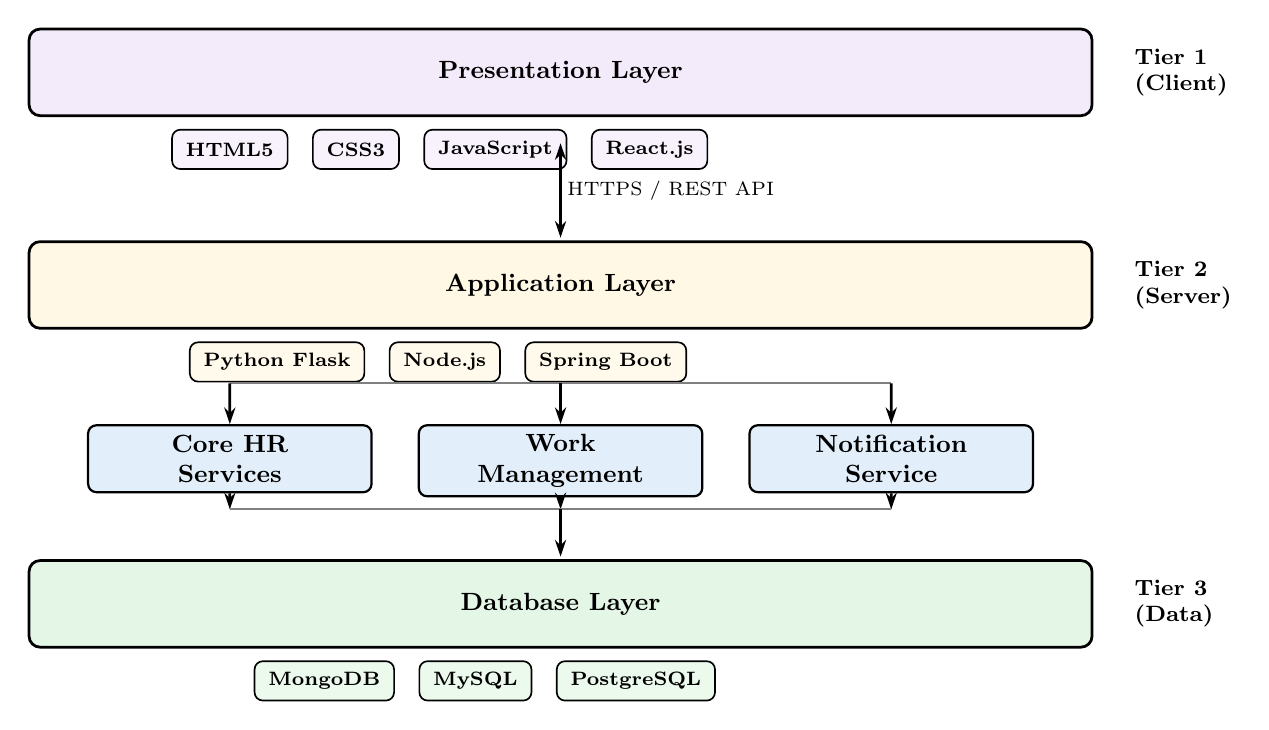
\begin{tikzpicture}[
  slab/.style={rectangle, draw=black, line width=1pt, rounded corners=4pt,
               minimum width=13.5cm, minimum height=1.1cm,
               align=center, font=\bfseries\small},
  badge/.style={rectangle, draw=black, line width=0.6pt, rounded corners=3pt,
                minimum height=0.5cm, inner xsep=5pt, inner ysep=2pt,
                font=\scriptsize\bfseries},
  submod/.style={rectangle, draw=black, line width=0.8pt, rounded corners=3pt,
                 minimum width=3.6cm, minimum height=0.85cm,
                 align=center, font=\small\bfseries},
  conn/.style={-{Stealth[length=6pt,width=4pt]}, line width=1pt},
  dconn/.style={{Stealth[length=6pt,width=4pt]}-{Stealth[length=6pt,width=4pt]}, line width=1pt}
]

% ---- TIER 1: Presentation ----
\node[slab, fill=nodepurple!50] (T1) at (0,0) {Presentation Layer};
\node[badge, fill=nodepurple!30, below=0.15cm of T1.south, xshift=-4.2cm] (bH) {HTML5};
\node[badge, fill=nodepurple!30, right=0.3cm of bH] (bC) {CSS3};
\node[badge, fill=nodepurple!30, right=0.3cm of bC] (bJ) {JavaScript};
\node[badge, fill=nodepurple!30, right=0.3cm of bJ] (bR) {React.js};

% ---- Arrow T1 -> T2 ----
\draw[dconn] (0,-0.9) -- node[right, font=\scriptsize, fill=white, inner sep=2pt]{HTTPS / REST API} (0,-2.1);

% ---- TIER 2: Application ----
\node[slab, fill=nodeyellow!55] (T2) at (0,-2.7) {Application Layer};
\node[badge, fill=nodeyellow!40, below=0.15cm of T2.south, xshift=-3.6cm] (bPy) {Python Flask};
\node[badge, fill=nodeyellow!40, right=0.3cm of bPy] (bNo) {Node.js};
\node[badge, fill=nodeyellow!40, right=0.3cm of bNo] (bSp) {Spring Boot};

% ---- Sub-module boxes ----
\node[submod, fill=nodeblue!55, below=1.2cm of T2, xshift=-4.2cm] (mHR)   {Core HR\\Services};
\node[submod, fill=nodeblue!55, below=1.2cm of T2]                (mWork) {Work\\Management};
\node[submod, fill=nodeblue!55, below=1.2cm of T2, xshift= 4.2cm] (mNote) {Notification\\Service};

% Bus: T2 -> module tops
\draw[line width=0.7pt, black!50] (-4.2,-3.95) -- (4.2,-3.95);
\draw[conn] (-4.2,-3.95) -- (mHR.north);
\draw[conn] (0,   -3.95) -- (mWork.north);
\draw[conn] ( 4.2,-3.95) -- (mNote.north);

% Bus: module bottoms -> T3
\draw[conn] (mHR.south)   -- (-4.2,-5.55);
\draw[conn] (mWork.south) -- (0,   -5.55);
\draw[conn] (mNote.south) -- ( 4.2,-5.55);
\draw[line width=0.7pt, black!50] (-4.2,-5.55) -- (4.2,-5.55);
\draw[conn] (0,-5.55) -- (0,-6.15);

% ---- TIER 3: Database ----
\node[slab, fill=nodegreen!50] (T3) at (0,-6.75) {Database Layer};
\node[badge, fill=nodegreen!35, below=0.15cm of T3.south, xshift=-3.0cm] (bM) {MongoDB};
\node[badge, fill=nodegreen!35, right=0.3cm of bM] (bMy) {MySQL};
\node[badge, fill=nodegreen!35, right=0.3cm of bMy] (bPG) {PostgreSQL};

% ---- Tier labels (right margin) ----
\node[font=\footnotesize\bfseries, right=0.4cm of T1.east, align=left] {Tier 1\\(Client)};
\node[font=\footnotesize\bfseries, right=0.4cm of T2.east, align=left] {Tier 2\\(Server)};
\node[font=\footnotesize\bfseries, right=0.4cm of T3.east, align=left] {Tier 3\\(Data)};

\end{tikzpicture}
\caption{Three-Tier System Architecture with Technology Stack}
\end{figure}

\section{Software and Hardware Requirements}

\textbf{Software Requirements}
\begin{itemize}
  \item \textbf{Operating System:} Windows, Linux, or macOS
  \item \textbf{Programming Languages:} Python, Java, or JavaScript
  \item \textbf{Frontend Tech Stack:} HTML5, CSS3, JavaScript
  \item \textbf{Backend Framework:} Python Flask, Node.js, or Java Spring Boot
  \item \textbf{Database:} MongoDB (with MongoDB Compass GUI)
  \item \textbf{Development Tools:} VS Code, Chrome/Firefox, Postman
\end{itemize}

\textbf{Hardware Requirements}
\begin{itemize}
  \item \textbf{Processor:} Dual-core processor (or better)
  \item \textbf{RAM:} 4 GB minimum (8 GB recommended)
  \item \textbf{Storage:} Minimum 10 GB free space
  \item \textbf{Network:} Active internet connection for cloud hosting and dependency installation
\end{itemize}

\section{Dependencies}
\begin{itemize}
  \item Running instance of the chosen database server (e.g., MongoDB Daemon).
  \item Valid installation of the backend runtime (e.g., Python 3.x or Node.js).
  \item Libraries and drivers installed via \texttt{pip} or \texttt{npm}.
  \item Web browser for accessing the application interface.
\end{itemize}

\section{Constraints}
\begin{itemize}
  \item \textbf{Resources:} Project is bound by limited development time and budget.
  \item \textbf{Storage:} Maximum database size depends on host server capacity.
  \item \textbf{Security:} Sensitive modules are restricted by predefined user roles.
  \item \textbf{Environment:} A stable internet connection is required for cloud deployment.
  \item \textbf{Hardware Limitations:} Physical biometric integration is outside current capabilities.
\end{itemize}

\section{Assumptions}
\begin{itemize}
  \item End-users will possess basic computer literacy and internet navigation skills.
  \item The HR department will provide accurate and validated initial data.
  \item Each employee will be assigned a globally unique Employee ID.
  \item The host server will maintain standard uptime with regular automated backups.
  \item Users will adhere to organisational security policies regarding password sharing.
  \item The modular architecture will allow feature expansions without disrupting core operations.
\end{itemize}

% ============================================================
\chapter{Next Lab Tasks: Design \& Testing}
% ============================================================

\section{SRS Part 2: Design Documents}

\subsection{High-Level Design (HLD)}

\subsubsection{Data Flow Diagram --- Level 0}

\begin{figure}[h!]
\centering
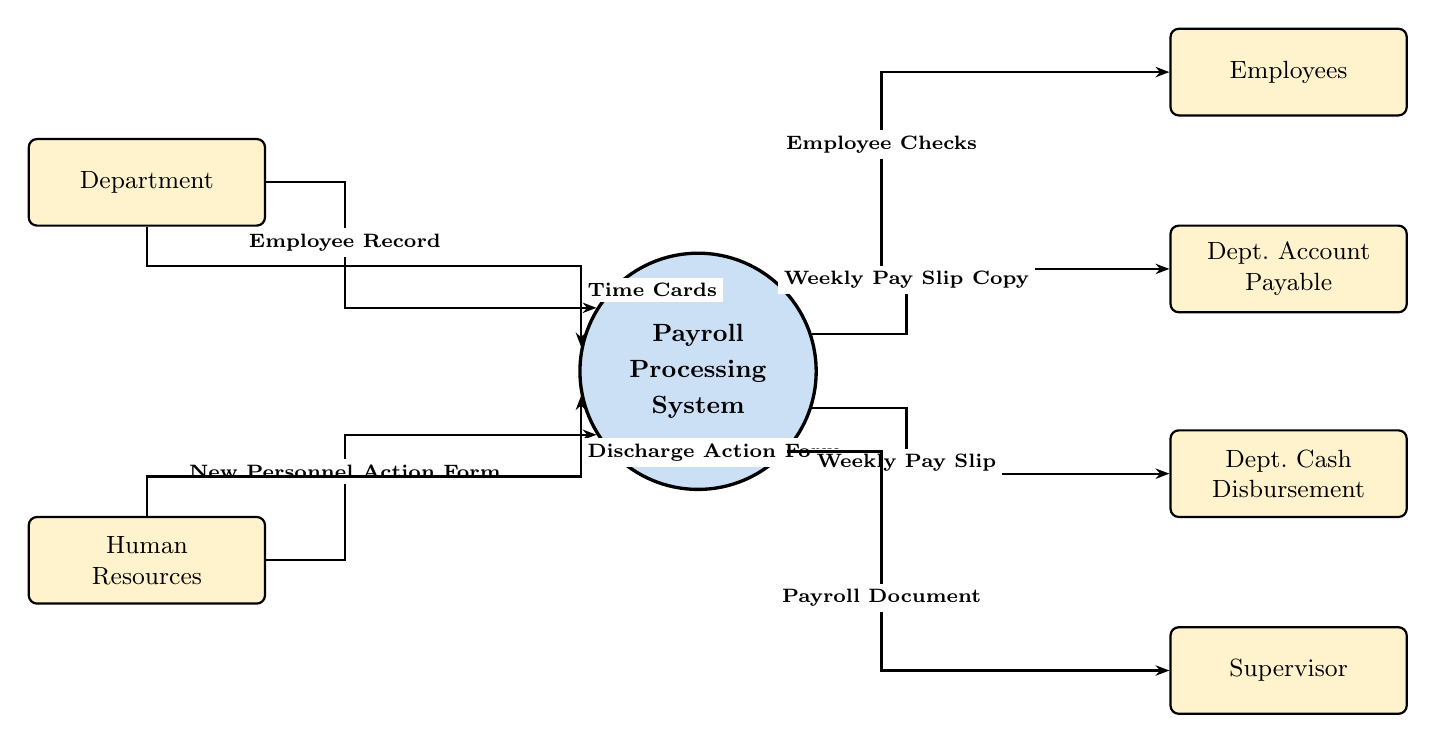
\begin{tikzpicture}[every node/.style={font=\small}]
  % Central process
  \node[dfdproc] (sys) at (0,0) {\textbf{Payroll}\\[2pt]\textbf{Processing}\\[2pt]\textbf{System}};
  % Left entities
  \node[dfdent] (dept) at (-7,  2.4) {Department};
  \node[dfdent] (hr)   at (-7, -2.4) {Human\\Resources};
  % Right entities --- 2.0cm gap each
  \node[dfdent] (emp) at (7.5,  3.8) {Employees};
  \node[dfdent] (dap) at (7.5,  1.3) {Dept.\ Account\\Payable};
  \node[dfdent] (dcd) at (7.5, -1.3) {Dept.\ Cash\\Disbursement};
  \node[dfdent] (sup) at (7.5, -3.8) {Supervisor};
  % Inputs: left -> system via elbow routing
  \draw[-{Stealth[length=5pt]},thick,draw=black]
    (dept.east) -- ++(1.0,0) |-
    node[pos=0.3,above,font=\scriptsize\bfseries,fill=white,inner sep=2pt]{Employee Record}
    (sys.148);
  \draw[-{Stealth[length=5pt]},thick,draw=black]
    (dept.south) -- ++(0,-0.5) -|
    node[pos=0.65,right,font=\scriptsize\bfseries,fill=white,inner sep=2pt]{Time Cards}
    (sys.168);
  \draw[-{Stealth[length=5pt]},thick,draw=black]
    (hr.east) -- ++(1.0,0) |-
    node[pos=0.3,above,font=\scriptsize\bfseries,fill=white,inner sep=2pt]{New Personnel Action Form}
    (sys.212);
  \draw[-{Stealth[length=5pt]},thick,draw=black]
    (hr.north) -- ++(0,0.5) -|
    node[pos=0.65,right,font=\scriptsize\bfseries,fill=white,inner sep=2pt]{Discharge Action Form}
    (sys.192);
  % Outputs: system -> right via elbow routing
  \draw[-{Stealth[length=5pt]},thick,draw=black]
    (sys.42) -- ++(1.2,0) |-
    node[pos=0.3,above,font=\scriptsize\bfseries,fill=white,inner sep=2pt]{Employee Checks}
    (emp.west);
  \draw[-{Stealth[length=5pt]},thick,draw=black]
    (sys.18) -- ++(1.2,0) |-
    node[pos=0.3,above,font=\scriptsize\bfseries,fill=white,inner sep=2pt]{Weekly Pay Slip Copy}
    (dap.west);
  \draw[-{Stealth[length=5pt]},thick,draw=black]
    (sys.342) -- ++(1.2,0) |-
    node[pos=0.3,below,font=\scriptsize\bfseries,fill=white,inner sep=2pt]{Weekly Pay Slip}
    (dcd.west);
  \draw[-{Stealth[length=5pt]},thick,draw=black]
    (sys.318) -- ++(1.2,0) |-
    node[pos=0.3,below,font=\scriptsize\bfseries,fill=white,inner sep=2pt]{Payroll Document}
    (sup.west);
\end{tikzpicture}
\caption{Level 0 Data Flow Diagram --- Payroll Processing System}
\end{figure}

\begin{itemize}
  \item \textbf{Core HR Module:} Handles Employees, Leaves, Attendance, and Payroll.
  \item \textbf{Work Management Module:} Handles Tasks, Boards, and Projects.
  \item \textbf{Event Engine:} Listens to HR events (e.g., Leave Approval) and triggers cross-functional actions in the Work Module (e.g., Task Reassignment).
\end{itemize}

\subsubsection{Use Case Diagram}

\begin{figure}[h!]
\centering
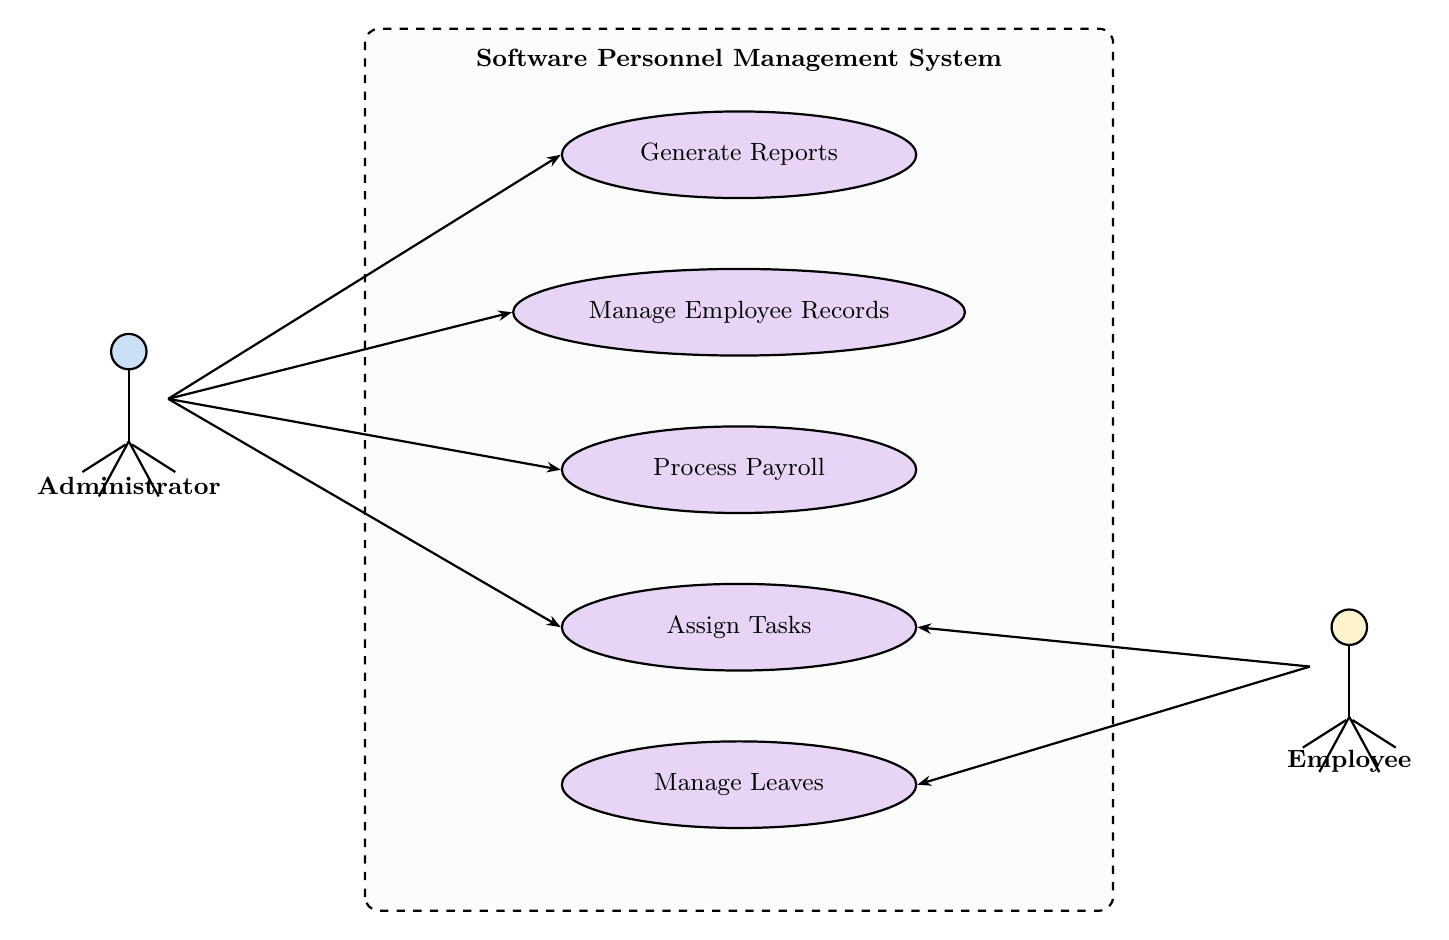
\begin{tikzpicture}
  % System boundary
  \draw[draw=black,thick,dashed,rounded corners=5pt,fill=softgray,fill opacity=0.3]
    (-4,-5.6) rectangle (5.5,5.6);
  \node[font=\bfseries\small] at (0.75,5.2)
    {Software Personnel Management System};
  % Use cases --- 2.0cm vertical spacing
  \node[ucbox] (uc1) at (0.75,  4.0) {Generate Reports};
  \node[ucbox] (uc2) at (0.75,  2.0) {Manage Employee Records};
  \node[ucbox] (uc3) at (0.75,  0.0) {Process Payroll};
  \node[ucbox] (uc4) at (0.75, -2.0) {Assign Tasks};
  \node[ucbox] (uc5) at (0.75, -4.0) {Manage Leaves};
  % Administrator stick figure (left)
  \node[circle,draw,thick,minimum size=0.45cm,fill=nodeblue] (h1) at (-7.0,1.5) {};
  \draw[thick] (h1.south) -- ++(0,-0.9) coordinate (b1);
  \draw[thick] (b1)++(-0.04,-0.04) -- ++(-0.55,-0.35);
  \draw[thick] (b1)++( 0.04,-0.04) -- ++( 0.55,-0.35);
  \draw[thick] (b1) -- ++(-0.38,-0.7);
  \draw[thick] (b1) -- ++( 0.38,-0.7);
  \node[font=\small\bfseries] at (-7.0,-0.2) {Administrator};
  \coordinate (admin) at (-6.5,0.9);
  % Employee stick figure (right)
  \node[circle,draw,thick,minimum size=0.45cm,fill=nodeyellow] (h2) at (8.5,-2.0) {};
  \draw[thick] (h2.south) -- ++(0,-0.9) coordinate (b2);
  \draw[thick] (b2)++(-0.04,-0.04) -- ++(-0.55,-0.35);
  \draw[thick] (b2)++( 0.04,-0.04) -- ++( 0.55,-0.35);
  \draw[thick] (b2) -- ++(-0.38,-0.7);
  \draw[thick] (b2) -- ++( 0.38,-0.7);
  \node[font=\small\bfseries] at (8.5,-3.7) {Employee};
  \coordinate (employee) at (8.0,-2.5);
  % Arrows
  \draw[msgfwd] (admin) -- (uc1.west);
  \draw[msgfwd] (admin) -- (uc2.west);
  \draw[msgfwd] (admin) -- (uc3.west);
  \draw[msgfwd] (admin) -- (uc4.west);
  \draw[msgfwd] (employee) -- (uc4.east);
  \draw[msgfwd] (employee) -- (uc5.east);
\end{tikzpicture}
\caption{Use Case Diagram --- Software Personnel Management System}
\end{figure}

\subsubsection{Activity Diagram}

\begin{figure}[htbp]
\centering
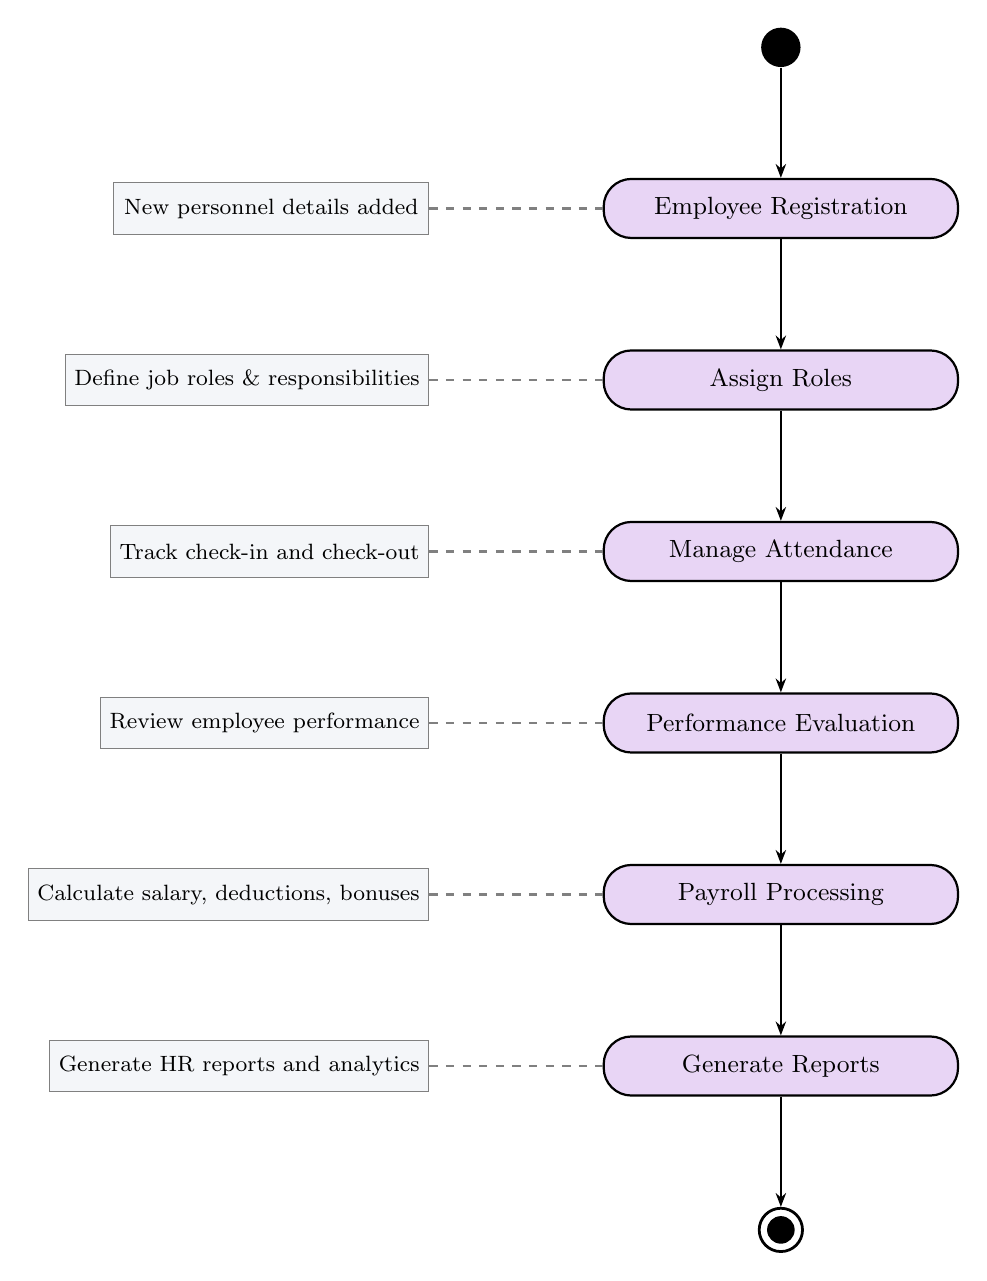
\begin{tikzpicture}[node distance=1.4cm]
  \node[circle,fill=black,minimum size=0.5cm] (start) at (0,0) {};
  \node[actbox,below=of start] (a1) {Employee Registration};
  \node[actbox,below=of a1]    (a2) {Assign Roles};
  \node[actbox,below=of a2]    (a3) {Manage Attendance};
  \node[actbox,below=of a3]    (a4) {Performance Evaluation};
  \node[actbox,below=of a4]    (a5) {Payroll Processing};
  \node[actbox,below=of a5]    (a6) {Generate Reports};
  \node[circle,draw=black,line width=1pt,minimum size=0.55cm,below=of a6] (endout) {};
  \node[circle,fill=black,minimum size=0.35cm] at (endout) {};
  % Flow
  \draw[msgfwd] (start)--(a1); \draw[msgfwd] (a1)--(a2);
  \draw[msgfwd] (a2)--(a3);    \draw[msgfwd] (a3)--(a4);
  \draw[msgfwd] (a4)--(a5);    \draw[msgfwd] (a5)--(a6);
  \draw[msgfwd] (a6)--(endout);
  % Notes
  \node[notebox,left=2.2cm of a1] (n1) {New personnel details added};
  \node[notebox,left=2.2cm of a2] (n2) {Define job roles \& responsibilities};
  \node[notebox,left=2.2cm of a3] (n3) {Track check-in and check-out};
  \node[notebox,left=2.2cm of a4] (n4) {Review employee performance};
  \node[notebox,left=2.2cm of a5] (n5) {Calculate salary, deductions, bonuses};
  \node[notebox,left=2.2cm of a6] (n6) {Generate HR reports and analytics};
  \foreach \n/\a in {n1/a1,n2/a2,n3/a3,n4/a4,n5/a5,n6/a6}{
    \draw[dashed,draw=black!50,thick] (\n.east)--(\a.west);
  }
\end{tikzpicture}
\caption{Activity Diagram --- Primary Personnel Workflow}
\end{figure}

\vspace{0.8cm}

\subsection{Low-Level Design (LLD)}
The LLD specifies classes, functions, and interfaces for the above modules, including specific APIs
for cross-module interactions (e.g., \texttt{generateOnboardingBoard(employeeId)} and
\texttt{flagTasksOnLeave(employeeId)}).

\subsubsection{Sequence Diagram --- Employee Flow}

\begin{figure}[htbp]
\centering
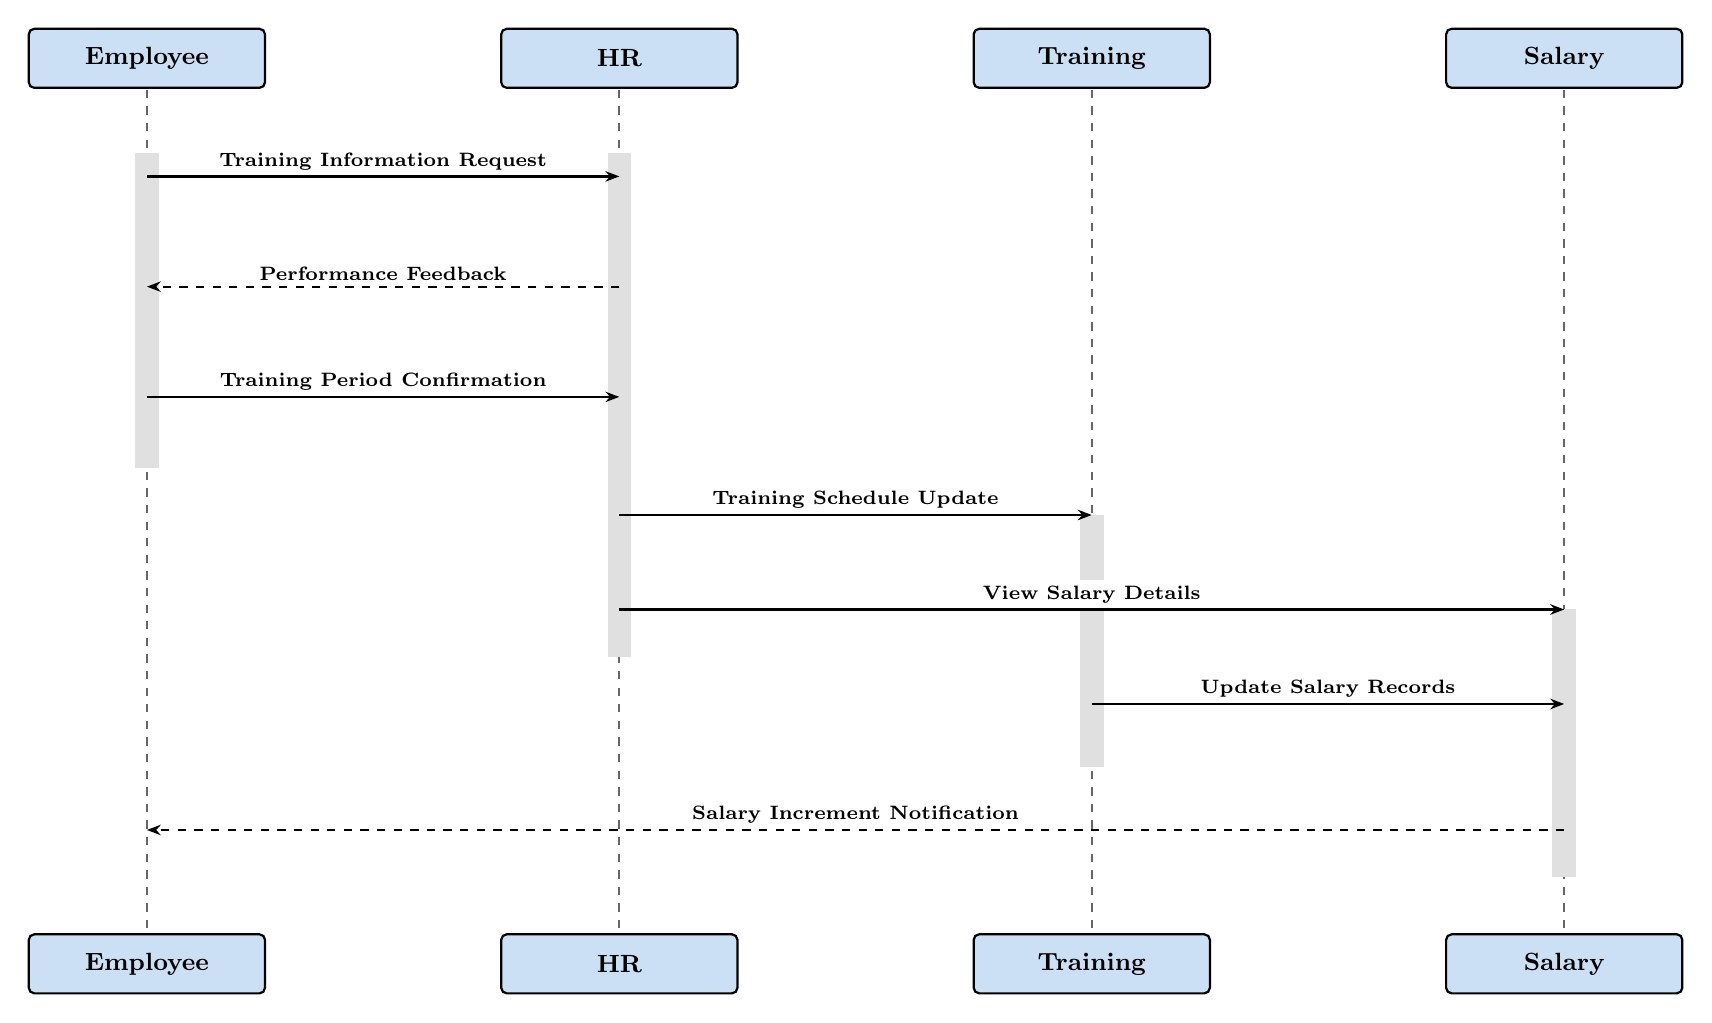
\begin{tikzpicture}
  % Column x-positions (6cm apart for breathing room)
  \def\xA{0}   % Employee
  \def\xB{6}   % HR
  \def\xC{12}  % Training
  \def\xD{18}  % Salary
  % Lifeline total height
  \def\yTop{0}
  \def\yBot{-11.5}
  % ---- Actor header boxes ----
  \node[actorbox, minimum width=3cm] (aEmp)   at (\xA, \yTop) {Employee};
  \node[actorbox, minimum width=3cm] (aHR)    at (\xB, \yTop) {HR};
  \node[actorbox, minimum width=3cm] (aTrain) at (\xC, \yTop) {Training};
  \node[actorbox, minimum width=3cm] (aSal)   at (\xD, \yTop) {Salary};
  % ---- Actor footer boxes ----
  \node[actorbox, minimum width=3cm] at (\xA, \yBot) {Employee};
  \node[actorbox, minimum width=3cm] at (\xB, \yBot) {HR};
  \node[actorbox, minimum width=3cm] at (\xC, \yBot) {Training};
  \node[actorbox, minimum width=3cm] at (\xD, \yBot) {Salary};
  % ---- Lifelines ----
  \draw[lifeline] (\xA,-0.4) -- (\xA,-11.1);
  \draw[lifeline] (\xB,-0.4) -- (\xB,-11.1);
  \draw[lifeline] (\xC,-0.4) -- (\xC,-11.1);
  \draw[lifeline] (\xD,-0.4) -- (\xD,-11.1);
  % ---- Activation boxes (thin filled rect on lifeline) ----
  \fill[black!12] (\xA-0.15,-1.2) rectangle (\xA+0.15,-5.2);
  \fill[black!12] (\xB-0.15,-1.2) rectangle (\xB+0.15,-7.6);
  \fill[black!12] (\xC-0.15,-5.8) rectangle (\xC+0.15,-9.0);
  \fill[black!12] (\xD-0.15,-7.0) rectangle (\xD+0.15,-10.4);
  % ---- Messages (1.4cm step) ----
  % 1: Emp -> HR
  \draw[msgfwd] (\xA,-1.5) -- (\xB,-1.5)
    node[midway, above, font=\scriptsize\bfseries, fill=white, inner sep=2pt]
    {Training Information Request};
  % 2: HR -> Emp (return)
  \draw[msgrtn] (\xB,-2.9) -- (\xA,-2.9)
    node[midway, above, font=\scriptsize\bfseries, fill=white, inner sep=2pt]
    {Performance Feedback};
  % 3: Emp -> HR
  \draw[msgfwd] (\xA,-4.3) -- (\xB,-4.3)
    node[midway, above, font=\scriptsize\bfseries, fill=white, inner sep=2pt]
    {Training Period Confirmation};
  % 4: HR -> Training
  \draw[msgfwd] (\xB,-5.8) -- (\xC,-5.8)
    node[midway, above, font=\scriptsize\bfseries, fill=white, inner sep=2pt]
    {Training Schedule Update};
  % 5: HR -> Salary
  \draw[msgfwd] (\xB,-7.0) -- (\xD,-7.0)
    node[midway, above, font=\scriptsize\bfseries, fill=white, inner sep=2pt]
    {View Salary Details};
  % 6: Training -> Salary
  \draw[msgfwd] (\xC,-8.2) -- (\xD,-8.2)
    node[midway, above, font=\scriptsize\bfseries, fill=white, inner sep=2pt]
    {Update Salary Records};
  % 7: Salary -> Emp (return)
  \draw[msgrtn] (\xD,-9.8) -- (\xA,-9.8)
    node[midway, above, font=\scriptsize\bfseries, fill=white, inner sep=2pt]
    {Salary Increment Notification};
\end{tikzpicture}
\caption{Sequence Diagram --- Training and Salary Processing}
\end{figure}

\vspace{1cm}

\subsubsection{Sequence Diagram --- Administrator Flow}

\begin{figure}[htbp]
\centering
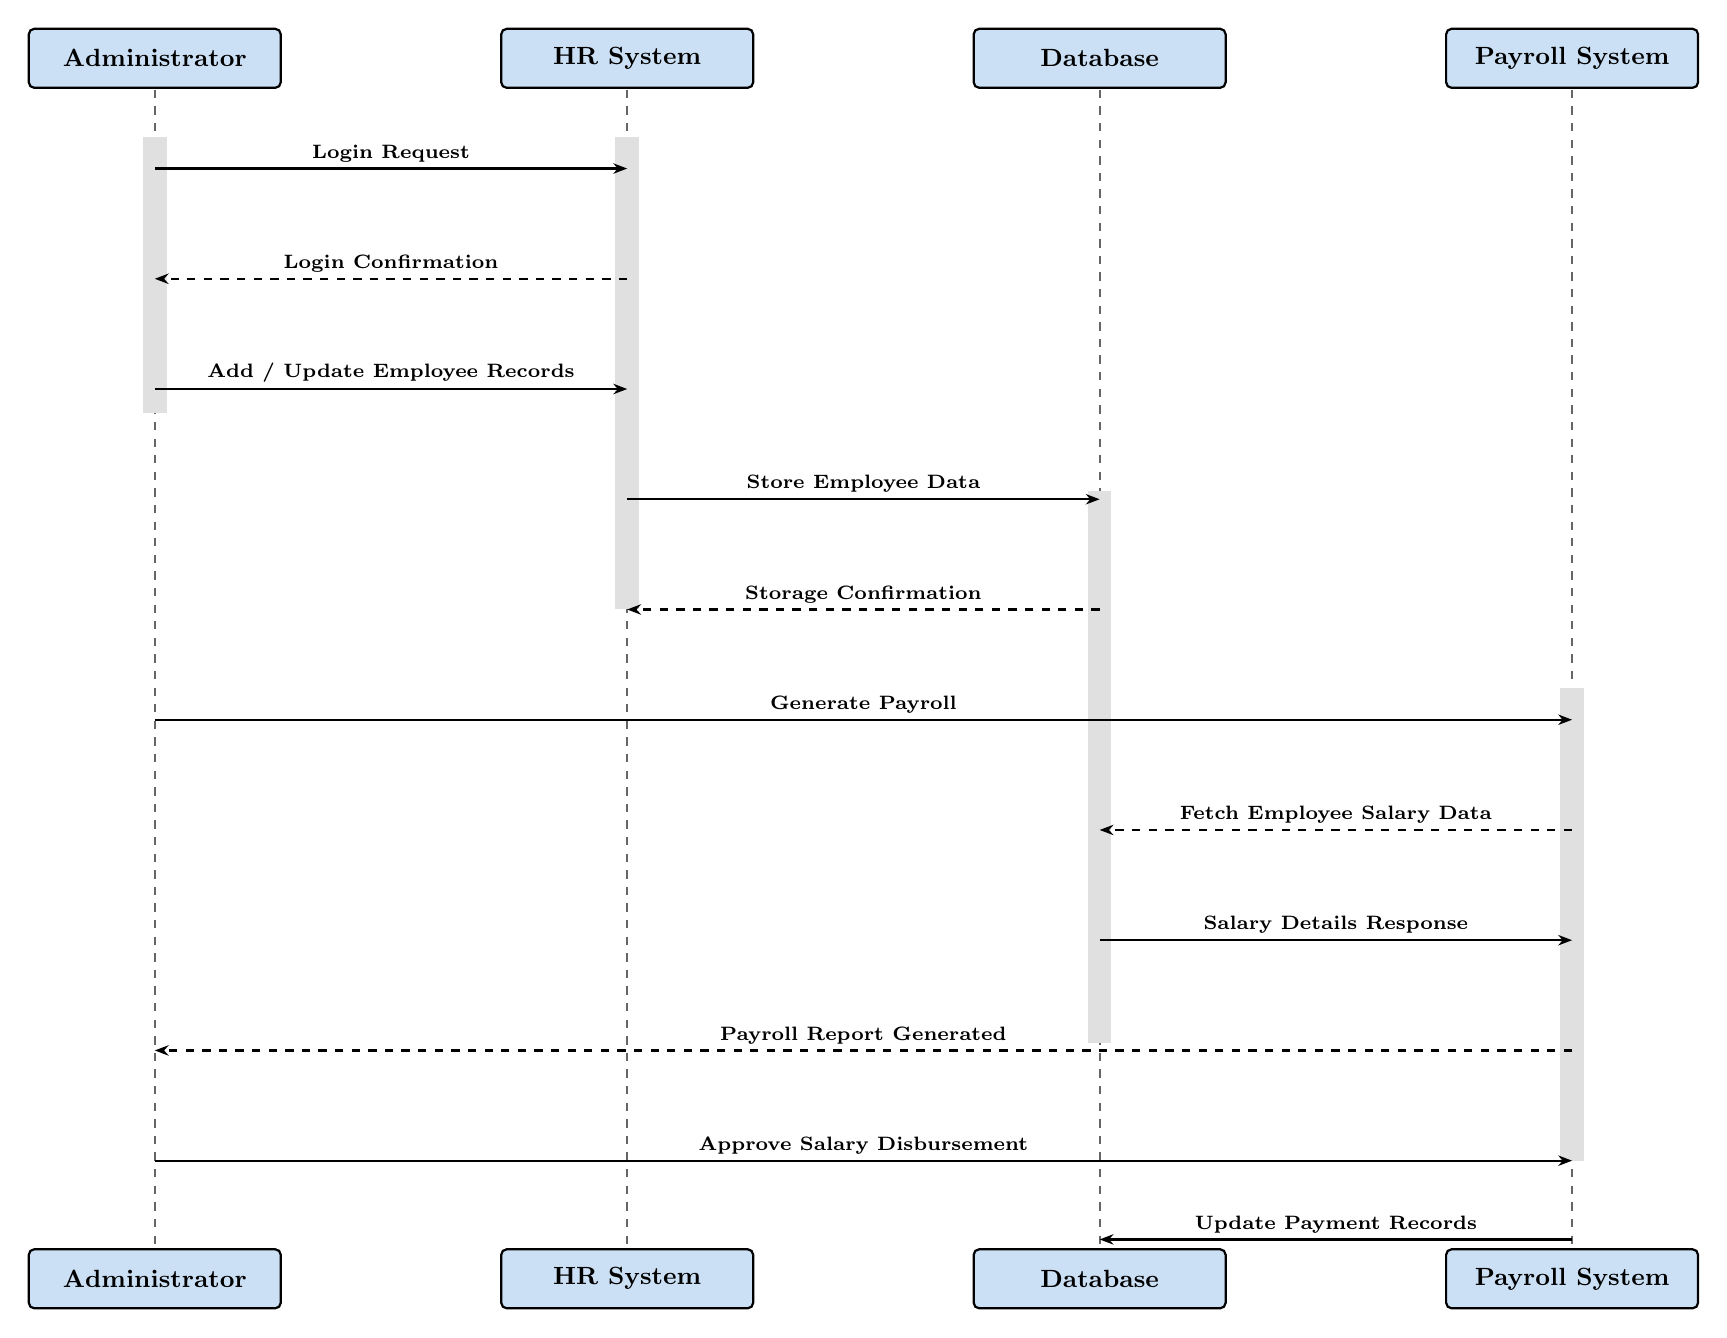
\begin{tikzpicture}
  % Column x-positions (6cm apart)
  \def\xA{0}   % Administrator
  \def\xB{6}   % HR System
  \def\xC{12}  % Database
  \def\xD{18}  % Payroll System
  % ---- Actor header boxes ----
  \node[actorbox, minimum width=3.2cm] at (\xA, 0) {Administrator};
  \node[actorbox, minimum width=3.2cm] at (\xB, 0) {HR System};
  \node[actorbox, minimum width=3.2cm] at (\xC, 0) {Database};
  \node[actorbox, minimum width=3.2cm] at (\xD, 0) {Payroll System};
  % ---- Actor footer boxes ----
  \node[actorbox, minimum width=3.2cm] at (\xA,-15.5) {Administrator};
  \node[actorbox, minimum width=3.2cm] at (\xB,-15.5) {HR System};
  \node[actorbox, minimum width=3.2cm] at (\xC,-15.5) {Database};
  \node[actorbox, minimum width=3.2cm] at (\xD,-15.5) {Payroll System};
  % ---- Lifelines ----
  \draw[lifeline] (\xA,-0.4) -- (\xA,-15.1);
  \draw[lifeline] (\xB,-0.4) -- (\xB,-15.1);
  \draw[lifeline] (\xC,-0.4) -- (\xC,-15.1);
  \draw[lifeline] (\xD,-0.4) -- (\xD,-15.1);
  % ---- Activation boxes ----
  \fill[black!12] (\xA-0.15,-1.0) rectangle (\xA+0.15,-4.5);
  \fill[black!12] (\xB-0.15,-1.0) rectangle (\xB+0.15,-7.0);
  \fill[black!12] (\xC-0.15,-5.5) rectangle (\xC+0.15,-12.5);
  \fill[black!12] (\xD-0.15,-8.0) rectangle (\xD+0.15,-14.0);
  % ---- Messages (1.4cm step) ----
  % 1
  \draw[msgfwd] (\xA,-1.4) -- (\xB,-1.4)
    node[midway,above,font=\scriptsize\bfseries,fill=white,inner sep=2pt]{Login Request};
  % 2
  \draw[msgrtn] (\xB,-2.8) -- (\xA,-2.8)
    node[midway,above,font=\scriptsize\bfseries,fill=white,inner sep=2pt]{Login Confirmation};
  % 3
  \draw[msgfwd] (\xA,-4.2) -- (\xB,-4.2)
    node[midway,above,font=\scriptsize\bfseries,fill=white,inner sep=2pt]{Add / Update Employee Records};
  % 4
  \draw[msgfwd] (\xB,-5.6) -- (\xC,-5.6)
    node[midway,above,font=\scriptsize\bfseries,fill=white,inner sep=2pt]{Store Employee Data};
  % 5
  \draw[msgrtn] (\xC,-7.0) -- (\xB,-7.0)
    node[midway,above,font=\scriptsize\bfseries,fill=white,inner sep=2pt]{Storage Confirmation};
  % 6
  \draw[msgfwd] (\xA,-8.4) -- (\xD,-8.4)
    node[midway,above,font=\scriptsize\bfseries,fill=white,inner sep=2pt]{Generate Payroll};
  % 7
  \draw[msgrtn] (\xD,-9.8) -- (\xC,-9.8)
    node[midway,above,font=\scriptsize\bfseries,fill=white,inner sep=2pt]{Fetch Employee Salary Data};
  % 8
  \draw[msgfwd] (\xC,-11.2) -- (\xD,-11.2)
    node[midway,above,font=\scriptsize\bfseries,fill=white,inner sep=2pt]{Salary Details Response};
  % 9
  \draw[msgrtn] (\xD,-12.6) -- (\xA,-12.6)
    node[midway,above,font=\scriptsize\bfseries,fill=white,inner sep=2pt]{Payroll Report Generated};
  % 10
  \draw[msgfwd] (\xA,-14.0) -- (\xD,-14.0)
    node[midway,above,font=\scriptsize\bfseries,fill=white,inner sep=2pt]{Approve Salary Disbursement};
  % 11
  \draw[msgfwd] (\xD,-15.0) -- (\xC,-15.0)
    node[midway,above,font=\scriptsize\bfseries,fill=white,inner sep=2pt]{Update Payment Records};
\end{tikzpicture}
\caption{Sequence Diagram --- Administrator: Payroll and Database Integration}
\end{figure}

\vspace{0.8cm}

\subsection{Database Design}
An Entity-Relationship (ER) model where the \texttt{User} table acts as a central foreign key
linking HR activities and Work items.
\begin{itemize}
  \item \textbf{Core Tables:} Users, Departments, Roles, Leaves, Attendance.
  \item \textbf{Work Tables:} Projects, Tasks, Kanban\_Boards.
\end{itemize}

\subsection{API Design}
RESTful API specifications connecting the front-end to backend services:
\begin{itemize}
  \item \texttt{POST /api/v1/onboarding} --- Triggers HR onboarding and board creation.
  \item \texttt{POST /api/v1/leaves/request} --- Submits a leave request.
  \item \texttt{GET /api/v1/users/\{id\}/workload} --- Fetches combined attendance and task load data.
\end{itemize}

\section{SRS Part 3: Testing Phase}

\subsection{Test Plan}
Outlines the overall testing strategy: unit testing for individual modules, integration testing
for the event engine (ensuring HR events trigger work events), and User Acceptance Testing (UAT)
with real-world scenarios.

\subsection{Test Cases}
\begin{itemize}
  \item \textbf{TC01 (Onboarding):} Verify that a new hire approval automatically creates an onboarding Kanban board with default tasks.
  \item \textbf{TC02 (Leave Integration):} Verify that an approved leave request correctly flags the user's active tasks and notifies their manager.
  \item \textbf{TC03 (Permissions):} Verify that a manager can only view tasks of employees within their reporting hierarchy.
\end{itemize}

\subsection{Test Scripts}
\begin{itemize}
  \item \textbf{Frontend:} Cypress or Selenium for end-to-end UI flows.
  \item \textbf{Backend:} Jest, Mocha, or PyTest for API and unit-level validation.
\end{itemize}

\subsection{Test Data}
Creation of mock employee records (names, IDs, departments), sample project tasks, sample leave
requests, and dummy payroll data to simulate and validate real-world scenarios in the staging
environment.

\subsection{Defect Tracking}
A formalised process for logging and tracking bugs found during testing. Defects will be
categorised by severity (\textit{Critical, High, Medium, Low}) and linked back to specific
failed test cases.

\subsection{Traceability Matrix}
A matrix mapping Functional Requirements (e.g., \textit{FR1: Onboarding integration}) to Design
Components (API: \texttt{/onboarding}) and corresponding Test Cases (\textbf{TC01}), ensuring
100\% requirement coverage throughout the development lifecycle.

\subsection{Test Summary}
A final report generated after the testing phase concludes, detailing the number of test cases
executed, passed, and failed, along with an overall software quality assessment prior to
production deployment.

\end{document}
